%------------------------------------------------
%----------------------------------------------------------------------------------------
\section{DWARF}
%----------------------------------------------------------------------------------------
%------------------------------------------------

\begin{frame}{DWARF}
    \begin{itemize}
	    \item Debugging with Attributed Record Formats(DWARF)
	    \item Debug information format
	    \item Executable and Linkable Format(ELF)
    \end{itemize}
\end{frame}

%------------------------------------------------
%------------------------------------------------

\begin{frame}{DWARF Sections}
	\begin{figure}
		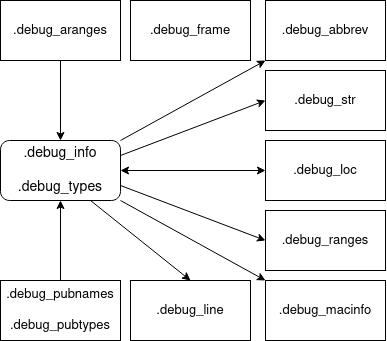
\includegraphics[width=0.9\textwidth,height=0.48\textwidth,keepaspectratio]{dwarf-sections.png}
	\end{figure}
\end{frame}

%------------------------------------------------
%------------------------------------------------

\begin{frame}{Debug Information Entry(DIE)}
	\begin{itemize}
	    \item DebugInformation Entry(DIE).
	    \item DWARF Attributes.
	    \item DWARF DIE example from the .debug\_info section.
	\end{itemize}
	\begin{figure}
		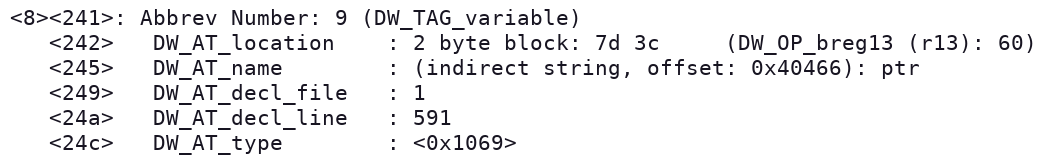
\includegraphics[width=0.9\textwidth,height=0.48\textwidth,keepaspectratio]{dwarf-die.png}
	\end{figure}
\end{frame}

%------------------------------------------------
%------------------------------------------------

\begin{frame}{Compilation unit}
	\begin{itemize}
		\item Computer program is devieded into compilation units.
		\item Each compilation unit contains a DIE tree.
	\end{itemize}
\end{frame}

%------------------------------------------------
%------------------------------------------------

\begin{frame}{Compilation unit}
	\begin{figure}
		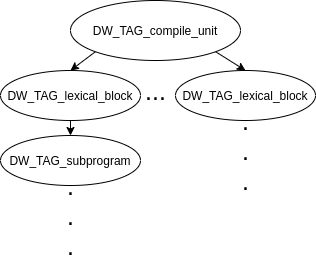
\includegraphics[width=0.9\textwidth,height=0.48\textwidth,keepaspectratio]{die-tree.png}
	\end{figure}
\end{frame}

%------------------------------------------------
%------------------------------------------------

\begin{frame}{Evaluating a variable}
    \begin{itemize}
        \item Two parts to evaluating a variable:
    	\begin{itemize}
    	    \item Finding the location of the variable
    	    \item Parsing the value into the correct type
    	\end{itemize}
    \end{itemize}
\end{frame}

%------------------------------------------------
%------------------------------------------------

\begin{frame}{Evaluating the location of a variable}
    \begin{itemize}
        \item Two parts to evaluating a variable:
        \item Two parts to evaluating a variable:
    \end{itemize}
\end{frame}

%------------------------------------------------
%------------------------------------------------

\begin{frame}{Evaluating the location of a variable}
	\begin{figure}
		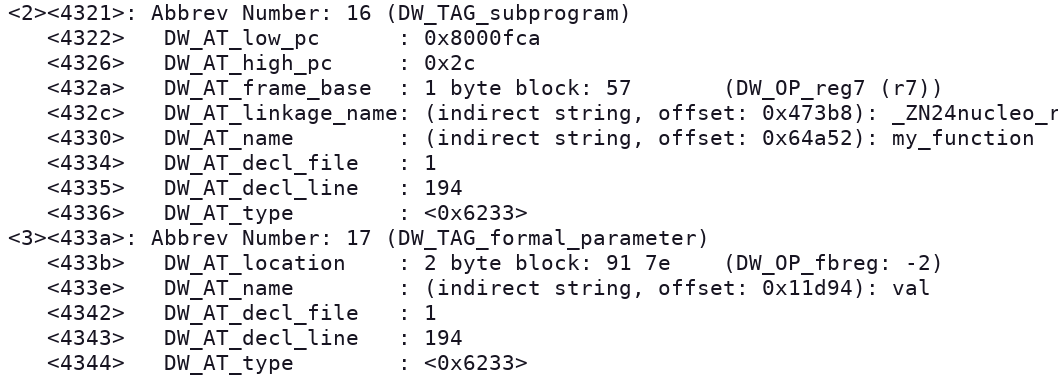
\includegraphics[width=0.9\textwidth,height=0.48\textwidth,keepaspectratio]{subprogram-example.png}
	\end{figure}
\end{frame}

%------------------------------------------------
%------------------------------------------------

\begin{frame}{Parsing the type of a variable}
	\begin{figure}
		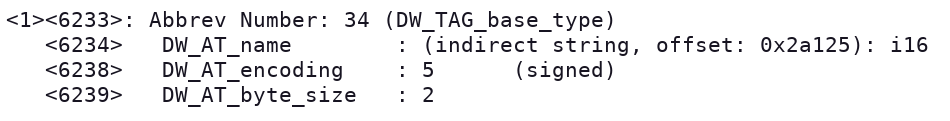
\includegraphics[width=0.9\textwidth,height=0.48\textwidth,keepaspectratio]{basetype-example.png}
	\end{figure}
\end{frame}

%------------------------------------------------
%------------------------------------------------

\begin{frame}{Virtually Unwinding Call Stack}
    \begin{itemize}
        \item Lorem ipsum dolor sit amet, consectetur adipiscing elit
        \item Aliquam blandit faucibus nisi, sit amet dapibus enim tempus eu
        \item Nulla commodo, erat quis gravida posuere, elit lacus lobortis est, quis porttitor odio mauris at libero
        \item Nam cursus est eget velit posuere pellentesque
        \item Vestibulum faucibus velit a augue condimentum quis convallis nulla gravida
    \end{itemize}
\end{frame}

%------------------------------------------------

